% Options for packages loaded elsewhere
% Options for packages loaded elsewhere
\PassOptionsToPackage{unicode}{hyperref}
\PassOptionsToPackage{hyphens}{url}
\PassOptionsToPackage{dvipsnames,svgnames,x11names}{xcolor}
%
\documentclass[
  letterpaper,
  DIV=11,
  numbers=noendperiod,
  oneside]{scrartcl}
\usepackage{xcolor}
\usepackage[left=1in,marginparwidth=2.0666666666667in,textwidth=4.1333333333333in,marginparsep=0.3in]{geometry}
\usepackage{amsmath,amssymb}
\setcounter{secnumdepth}{-\maxdimen} % remove section numbering
\usepackage{iftex}
\ifPDFTeX
  \usepackage[T1]{fontenc}
  \usepackage[utf8]{inputenc}
  \usepackage{textcomp} % provide euro and other symbols
\else % if luatex or xetex
  \usepackage{unicode-math} % this also loads fontspec
  \defaultfontfeatures{Scale=MatchLowercase}
  \defaultfontfeatures[\rmfamily]{Ligatures=TeX,Scale=1}
\fi
\usepackage{lmodern}
\ifPDFTeX\else
  % xetex/luatex font selection
\fi
% Use upquote if available, for straight quotes in verbatim environments
\IfFileExists{upquote.sty}{\usepackage{upquote}}{}
\IfFileExists{microtype.sty}{% use microtype if available
  \usepackage[]{microtype}
  \UseMicrotypeSet[protrusion]{basicmath} % disable protrusion for tt fonts
}{}
\makeatletter
\@ifundefined{KOMAClassName}{% if non-KOMA class
  \IfFileExists{parskip.sty}{%
    \usepackage{parskip}
  }{% else
    \setlength{\parindent}{0pt}
    \setlength{\parskip}{6pt plus 2pt minus 1pt}}
}{% if KOMA class
  \KOMAoptions{parskip=half}}
\makeatother
% Make \paragraph and \subparagraph free-standing
\makeatletter
\ifx\paragraph\undefined\else
  \let\oldparagraph\paragraph
  \renewcommand{\paragraph}{
    \@ifstar
      \xxxParagraphStar
      \xxxParagraphNoStar
  }
  \newcommand{\xxxParagraphStar}[1]{\oldparagraph*{#1}\mbox{}}
  \newcommand{\xxxParagraphNoStar}[1]{\oldparagraph{#1}\mbox{}}
\fi
\ifx\subparagraph\undefined\else
  \let\oldsubparagraph\subparagraph
  \renewcommand{\subparagraph}{
    \@ifstar
      \xxxSubParagraphStar
      \xxxSubParagraphNoStar
  }
  \newcommand{\xxxSubParagraphStar}[1]{\oldsubparagraph*{#1}\mbox{}}
  \newcommand{\xxxSubParagraphNoStar}[1]{\oldsubparagraph{#1}\mbox{}}
\fi
\makeatother


\usepackage{longtable,booktabs,array}
\usepackage{calc} % for calculating minipage widths
% Correct order of tables after \paragraph or \subparagraph
\usepackage{etoolbox}
\makeatletter
\patchcmd\longtable{\par}{\if@noskipsec\mbox{}\fi\par}{}{}
\makeatother
% Allow footnotes in longtable head/foot
\IfFileExists{footnotehyper.sty}{\usepackage{footnotehyper}}{\usepackage{footnote}}
\makesavenoteenv{longtable}
\usepackage{graphicx}
\makeatletter
\newsavebox\pandoc@box
\newcommand*\pandocbounded[1]{% scales image to fit in text height/width
  \sbox\pandoc@box{#1}%
  \Gscale@div\@tempa{\textheight}{\dimexpr\ht\pandoc@box+\dp\pandoc@box\relax}%
  \Gscale@div\@tempb{\linewidth}{\wd\pandoc@box}%
  \ifdim\@tempb\p@<\@tempa\p@\let\@tempa\@tempb\fi% select the smaller of both
  \ifdim\@tempa\p@<\p@\scalebox{\@tempa}{\usebox\pandoc@box}%
  \else\usebox{\pandoc@box}%
  \fi%
}
% Set default figure placement to htbp
\def\fps@figure{htbp}
\makeatother





\setlength{\emergencystretch}{3em} % prevent overfull lines

\providecommand{\tightlist}{%
  \setlength{\itemsep}{0pt}\setlength{\parskip}{0pt}}



 


% load packages
\usepackage{geometry}
\usepackage{xcolor}
\usepackage{eso-pic}
\usepackage{fancyhdr}
\usepackage{sectsty}
\usepackage{fontspec}
\usepackage{titlesec}

%% Set page size with a wider right margin
\geometry{a4paper, total={170mm,257mm}, left=20mm, top=20mm, bottom=20mm, right=50mm}

%% Let's define some colours
\definecolor{light}{HTML}{E6E6FA}
\definecolor{highlight}{HTML}{800080}
\definecolor{dark}{HTML}{330033}

%% Let's add the border on the right hand side 
% \AddToShipoutPicture{% 
%     \AtPageLowerLeft{% 
%         \put(\LenToUnit{\dimexpr\paperwidth-3cm},0){% 
%             \color{light}\rule{3cm}{\LenToUnit\paperheight}%
%           }%
%      }%
%      % logo
%     \AtPageLowerLeft{% start the bar at the bottom right of the page
%         \put(\LenToUnit{\dimexpr\paperwidth-2.25cm},27.2cm){% move it to the top right
%             \color{light}
\includegraphics[width=1.5cm]{_extensions/nrennie/PrettyPDF/logo.png}
%           }%
%      }%
% }

%% Style the page number
\fancypagestyle{mystyle}{
  \fancyhf{}
  \renewcommand\headrulewidth{0pt}
  \fancyfoot[R]{\thepage}
  \fancyfootoffset{3.5cm}
}
\setlength{\footskip}{20pt}

%% style the chapter/section fonts
\chapterfont{\color{dark}\fontsize{20}{16.8}\selectfont}
\sectionfont{\color{dark}\fontsize{20}{16.8}\selectfont}
\subsectionfont{\color{dark}\fontsize{14}{16.8}\selectfont}
\titleformat{\subsection}
  {\sffamily\Large\bfseries}{\thesection}{1em}{}[{\titlerule[0.8pt]}]
  
% left align title
\makeatletter
\renewcommand{\maketitle}{\bgroup\setlength{\parindent}{0pt}
\begin{flushleft}
  {\sffamily\huge\textbf{\MakeUppercase{\@title}}} \vspace{0.3cm} \newline
  {\Large {\@subtitle}} \newline
  \@author
\end{flushleft}\egroup
}
\makeatother

%% Use some custom fonts
\setsansfont{Ubuntu}[
    Path=_extensions/nrennie/PrettyPDF/Ubuntu/,
    Scale=0.9,
    Extension = .ttf,
    UprightFont=*-Regular,
    BoldFont=*-Bold,
    ItalicFont=*-Italic,
    ]

\setmainfont{Ubuntu}[
    Path=_extensions/nrennie/PrettyPDF/Ubuntu/,
    Scale=0.9,
    Extension = .ttf,
    UprightFont=*-Regular,
    BoldFont=*-Bold,
    ItalicFont=*-Italic,
    ]
\KOMAoption{captions}{tableheading}
\makeatletter
\@ifpackageloaded{caption}{}{\usepackage{caption}}
\AtBeginDocument{%
\ifdefined\contentsname
  \renewcommand*\contentsname{Table of contents}
\else
  \newcommand\contentsname{Table of contents}
\fi
\ifdefined\listfigurename
  \renewcommand*\listfigurename{List of Figures}
\else
  \newcommand\listfigurename{List of Figures}
\fi
\ifdefined\listtablename
  \renewcommand*\listtablename{List of Tables}
\else
  \newcommand\listtablename{List of Tables}
\fi
\ifdefined\figurename
  \renewcommand*\figurename{Figure}
\else
  \newcommand\figurename{Figure}
\fi
\ifdefined\tablename
  \renewcommand*\tablename{Table}
\else
  \newcommand\tablename{Table}
\fi
}
\@ifpackageloaded{float}{}{\usepackage{float}}
\floatstyle{ruled}
\@ifundefined{c@chapter}{\newfloat{codelisting}{h}{lop}}{\newfloat{codelisting}{h}{lop}[chapter]}
\floatname{codelisting}{Listing}
\newcommand*\listoflistings{\listof{codelisting}{List of Listings}}
\makeatother
\makeatletter
\makeatother
\makeatletter
\@ifpackageloaded{caption}{}{\usepackage{caption}}
\@ifpackageloaded{subcaption}{}{\usepackage{subcaption}}
\makeatother
\makeatletter
\@ifpackageloaded{tcolorbox}{}{\usepackage[skins,breakable]{tcolorbox}}
\makeatother
\makeatletter
\@ifundefined{shadecolor}{\definecolor{shadecolor}{rgb}{.97, .97, .97}}{}
\makeatother
\makeatletter
\@ifundefined{codebgcolor}{\definecolor{codebgcolor}{named}{light}}{}
\makeatother
\makeatletter
\ifdefined\Shaded\renewenvironment{Shaded}{\begin{tcolorbox}[frame hidden, breakable, sharp corners, boxrule=0pt, colback={codebgcolor}, enhanced]}{\end{tcolorbox}}\fi
\makeatother
\makeatletter
\@ifpackageloaded{sidenotes}{}{\usepackage{sidenotes}}
\@ifpackageloaded{marginnote}{}{\usepackage{marginnote}}
\makeatother
\makeatletter
\@ifpackageloaded{fontawesome5}{}{\usepackage{fontawesome5}}
\makeatother
\usepackage{bookmark}
\IfFileExists{xurl.sty}{\usepackage{xurl}}{} % add URL line breaks if available
\urlstyle{same}
\hypersetup{
  pdftitle={Introduction to Film History},
  colorlinks=true,
  linkcolor={highlight},
  filecolor={Maroon},
  citecolor={Blue},
  urlcolor={highlight},
  pdfcreator={LaTeX via pandoc}}


\title{Introduction to Film History}
\author{}
\date{}
\begin{document}
\maketitle

\pagestyle{mystyle}


\pandocbounded{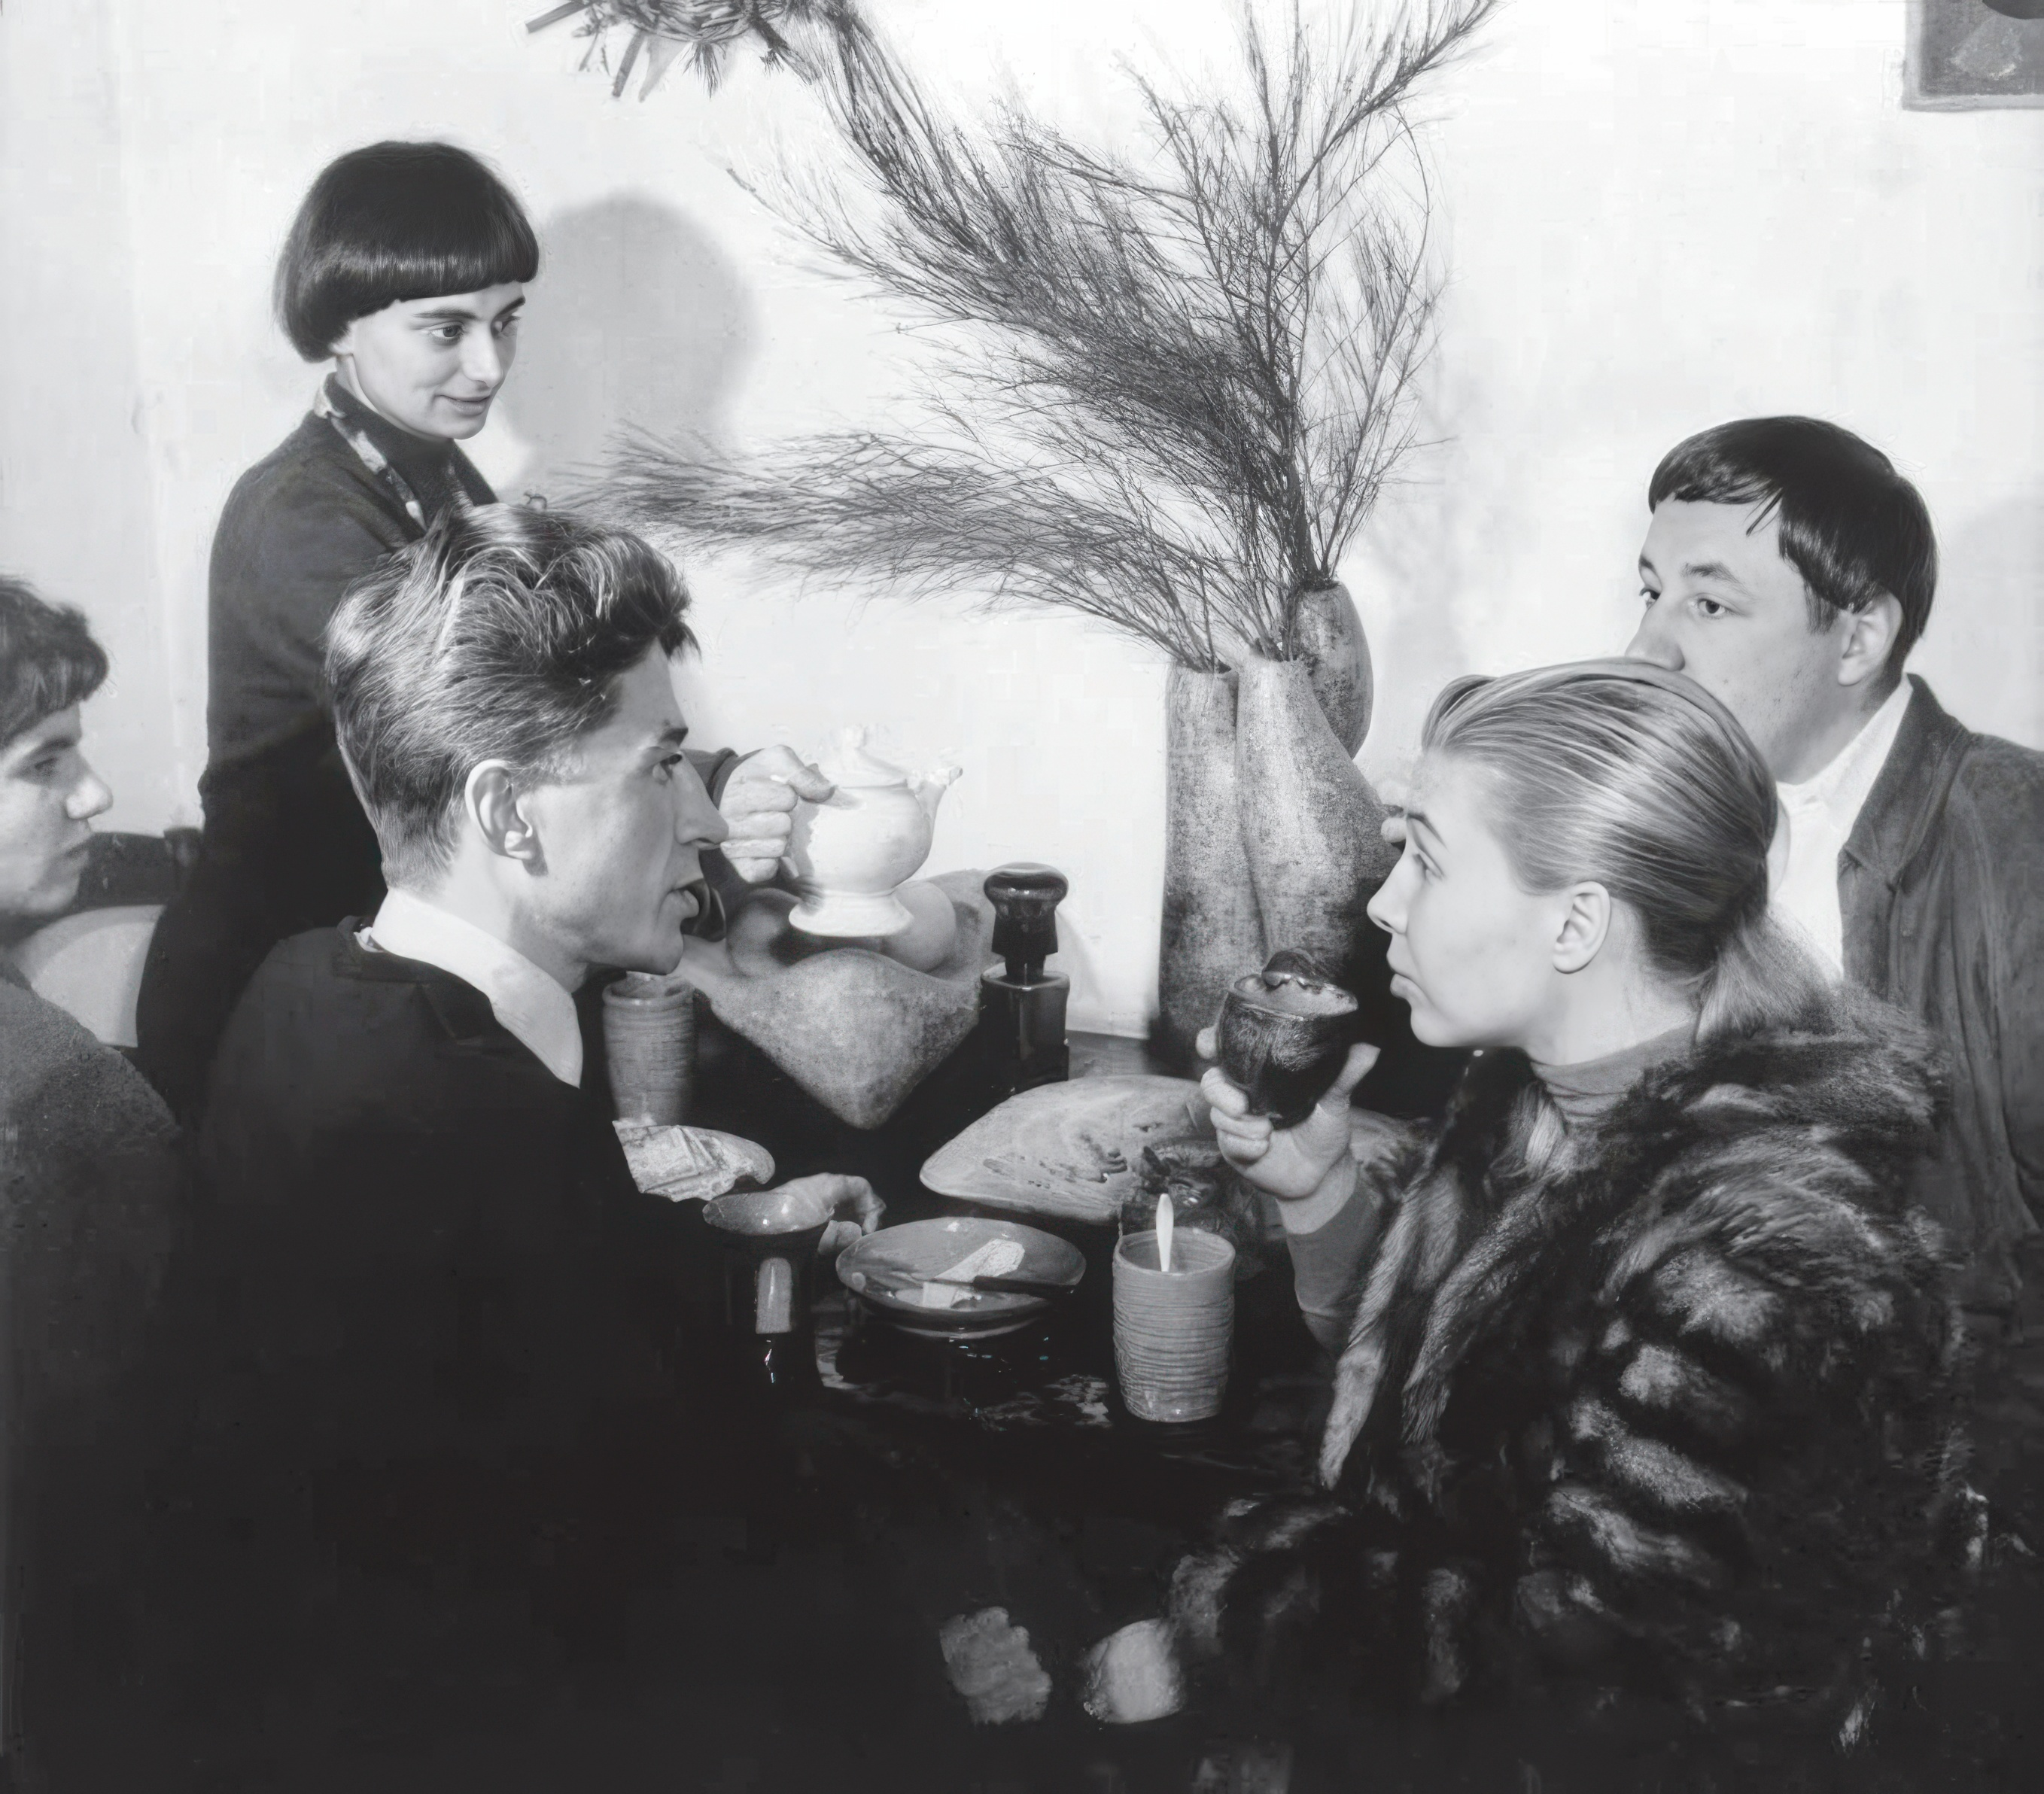
\includegraphics[keepaspectratio]{img/varda-resnais.jpg}}

\marginnote{\begin{footnotesize}

FILM 271-01-FA25\\
\href{https://keene.edu}{Keene State College}\\
Department of Film\\
Fall Semester 2025\\
Monday 10:00 a.m.-1:30 p.m.\\
Parker Hall: Drenan Auditorium\\
Instructor: Dr.~Martin Roberts\\
Office hours: Monday 16:00-17:00\\
Office location: Media Arts 124\\
\href{https://keene.instructure.com/courses/2474966}{Canvas}\\
\href{mailto:mdy45@usnh.edu}{\faIcon{envelope}} \textbar{}
\href{https://merveilles.town/@dokoissho}{\faIcon{mastodon}} \textbar{}
\href{https://github.com/mroberts1/}{\faIcon{github}} \textbar{}
\href{https://twitter.com/mroberts_vma}{\faIcon{twitter}}\\
\href{https://bsky.app/profile/dokoissho.bsky.social}{\faIcon{bluesky}}

\end{footnotesize}}

Agnès Varda (standing), Alain Resnais (left), Silvia Monfort and
Philippe Noiret (right) on the shoot of Varda's \emph{La Pointe Courte}
(1954)

\subsection{Course Goals}\label{course-goals}

To provide an introduction to :

\begin{itemize}
\tightlist
\item
  \textbf{film history}: motion pictures as a~\textbf{technology}, and
  filmmaking as an artistic and cultural~\textbf{practice}; the rise
  of~\textbf{national film industries}~and the star system;
  film~\textbf{genres}; major international~\textbf{film movements},
  including new waves, art cinema, and the avant-garde; and the
  development of cinema as a~\textbf{global}~artistic and cultural form.
\item
  \textbf{film analysis}, through its various dimensions of
  cinematography, mise-en-scène, editing, and sound.
\item
  \textbf{film culture}, including major~\textbf{institutions}~(film
  boards,~\emph{cinémathèques}, awards
  ceremonies),~\textbf{events}~(film festivals, screening
  series),~\textbf{publications}; and~\textbf{media}~(trailers, titles,
  posters).
\item
  \textbf{film theory}~as a research field and academic discipline,
  including major~\textbf{analytical frameworks}, **theoretical
  concepts, developing research topics, academic journals, etc.
\item
  the transformation of all aspects of filmmaking and global film
  culture by~\textbf{digital media}~technologies and
  the~\textbf{internet}, including production, post-production,
  distribution, exhibition, and restoration.
\end{itemize}

\subsection{Reading Assignments}\label{reading-assignments}

There is no textbook for this course.

Reading assignments will be available either as PDFs via Canvas or
online articles (follow links for access).

\begin{center}\rule{0.5\linewidth}{0.5pt}\end{center}

\subsection{Writing Assignments}\label{writing-assignments}

\textbf{Film Auteur} (1,500-2000 words / 6-8 pages double-spaced, with
bibliography)\\
Grading: Letter\\
At least three films by one of the following filmmakers:

\begin{itemize}
\tightlist
\item
  Michelangelo Antonioni
\item
  Shirley Clarke
\item
  Rainer Werner Fassbinder
\item
  Krzysztof Kieślowski
\item
  Stanley Kubrick
\item
  Joseph Losey
\item
  Louis Malle
\item
  Albert and David Maysles
\item
  Andrei Tarkovsky
\item
  Hiroshi Teshigahara
\item
  Jacques Tourneur
\item
  Agnès Varda
\item
  Charlotte Zwerin
\end{itemize}

\textbf{Film Movement} (1,000 words / 4 pages double-spaced)\\
Grading: Letter\\
An overview of an international film movement (pre-2000 only), involving
watching at least three films from the movement in question.

\textbf{Film Essay: Open Topic}\\
Grading: Letter\\
Possible topics: - Film studio (e.g.~Cinecittà) - Actor/Actress
(e.g.~Dirk Bogarde, Jeanne Moreau) - Cinematographer (e.g.~Nestor
Almendros)

\textbf{Reflection}\\
Grading: Complete/Incomplete\\
250-word reflection on the film screened that week, due by the following
class.\\
References to relevant sources encouraged and will get extra credit.\\
10 required; posted on Canvas weekly, from Week 3.

\textbf{Submission Formats} (any permitted)

\begin{itemize}
\tightlist
\item
  Written essay (see specific assignments for details). Submission:
  Canvas
\item
  Web essay (embedded images + clips). Submission: URL on Canvas
\item
  Video essay (edited clip compilation + titles + voiceover).
  Submission: upload to Google Drive, URL on Canvas
\end{itemize}

\begin{center}\rule{0.5\linewidth}{0.5pt}\end{center}

\subsection{Evaluation}\label{evaluation}

\begin{itemize}
\tightlist
\item
  Film Response (10 overall): 40\%
\item
  Movement Study: 20\%
\item
  Auteur Study: 20\%\\
\item
  Film Essay Project: 20\%
\end{itemize}

\begin{center}\rule{0.5\linewidth}{0.5pt}\end{center}

\subsection{Platforms}\label{platforms}

\href{https://www.criterion.com/}{Criterion}\\
\href{https://justwatch.io/}{Justwatch}\\
\href{https://letterboxd.com/}{Letterboxd}
\href{https://metrograph.com/}{Metrograph}\\
\href{https://mubi.com/}{Mubi}\\
\href{https://www.themoviedb.org/?language=en-US}{Movie Database}\\
\href{https://sundancenow.com}{Sundance Now}

\begin{center}\rule{0.5\linewidth}{0.5pt}\end{center}

\subsection{Resources}\label{resources}

\begin{itemize}
\tightlist
\item
  \href{https://cinemawavesblog.com/movements//}{Film Movements}
  (CinemaWaves website)
\item
  \href{https://www.movementsinfilm.com/}{Film Movements: A Beginner's
  Guide} (Movements in Film website)
\end{itemize}

\begin{center}\rule{0.5\linewidth}{0.5pt}\end{center}

\subsection{Films}\label{films}

\begin{itemize}
\tightlist
\item
  \emph{Cat People} (Jacques Tourneur, 1942)
\item
  \emph{Ascenseur pour l'échafaud} (\emph{Elevator to the Gallows},
  Louis Malle, 1958)
\item
  \emph{The Servant} (Joseph Losey, 1963)
\item
  \emph{Red Desert} (\emph{Il deserto rosso}, Michelangelo Antonioni,
  1964)
\item
  \emph{The Face of Another} (\emph{Tanin no kao}, Hiroshi Teshigahara,
  1966)
\item
  \emph{Portrait of Jason} (Shirley Clarke, 1967)
\item
  \emph{Black Panthers} (Agnès Varda, 1968)
\item
  \emph{Gimme Shelter} (Albert Maysles, David Maysles, Charlotte Zwerin,
  1970)
\item
  \emph{Killer of Sheep} (Charles Burnett, 1978)
\item
  \emph{The American Soldier} (\emph{Der amerikanische Soldat}, Rainer
  Werner Fassbinder, 1970)
\item
  \emph{Barry Lyndon} (Stanley Kubrick, 1975)
\item
  \emph{Stalker} (Andrei Tarkovsky, 1979)
\item
  \emph{Three Colours: Blue} (\emph{Trois couleurs: Bleu}, Krzysztof
  Kieślowski, 1993)
\end{itemize}

\begin{center}\rule{0.5\linewidth}{0.5pt}\end{center}

\subsection{Class Schedule}\label{class-schedule}

Week 1: Mon 25 Aug

Introduction: This Is Not A Survey Course

Screening: \emph{Cat People}

\begin{center}\rule{0.5\linewidth}{0.5pt}\end{center}

Week 2: Mon 1 Sept

NO CLASS (Labor Day)

\begin{center}\rule{0.5\linewidth}{0.5pt}\end{center}

Week 3: Mon 8 Sept

\textbf{Topic: Cat People}

Reading: - Daisuke Miyao, ``Cats Love Dark Places: Lighting in \emph{Cat
People}''

Screening: \emph{Elevator to the Gallows}

\begin{center}\rule{0.5\linewidth}{0.5pt}\end{center}

Week 4: Mon 15 Sept

\textbf{Nocturnal Cinema}

Reading: - Ginette Vincendeau, ``French Film Noir'' - Ginette
Vincendeau, ``Jeanne Moreau and the Actresses of the New Wave''

Screening: \emph{The Servant}

\begin{center}\rule{0.5\linewidth}{0.5pt}\end{center}

Week 5: Mon 22 Sept

\textbf{Red Hollywood}

Reading: - Selected chapters from David Caute, \emph{Joseph Losey: A
Revenge on Life}

Screening: \emph{Red Desert}

See also: \emph{Red Hollywood}

\begin{center}\rule{0.5\linewidth}{0.5pt}\end{center}

Week 6: Mon 29 Sept

\textbf{Art Cinema}

Reading:

\begin{itemize}
\tightlist
\item
  David Bordwell, ``The Art Cinema as a Mode of Film Practice''
\item
  Quaranta, ``\href{pdf/quaranta.pdf}{A Cinema of Boredom: Heidegger,
  Cinematic Time and Spectatorship}'' (\emph{Film-Philosophy}, 24.1
  (2020): 1-21)
\end{itemize}

Screening: \emph{The Face of Another}

\begin{center}\rule{0.5\linewidth}{0.5pt}\end{center}

Week 7: Mon 6 Oct

\textbf{Japanese New Wave}

Reading:

\begin{itemize}
\tightlist
\item
  Movements in Film on the
  \href{https://www.movementsinfilm.com/japanese-new-wave}{Japanese New
  Wave}
\item
  Cinemawaves on the
  \href{https://cinemawavesblog.com/movements/japanese-new-wave/}{Japanese
  New Wave}
\end{itemize}

See also:

Screening: \emph{Portrait of Jason}

\begin{center}\rule{0.5\linewidth}{0.5pt}\end{center}

Week 8 Mon 13 Oct

\textbf{Vérité}

Screening: \emph{Black Panthers}

\begin{center}\rule{0.5\linewidth}{0.5pt}\end{center}

Week 9: Mon 20 Oct

\textbf{Resistance}

Delphine Letort,
``\href{https://canvas.emerson.edu/courses/2040561/files/168958619?wrap=1}{Agnès
Varda: Filming the Black Panthers's Struggle}'' (\emph{L'Ordinaire des
Amériques}, 217 (2014))

Screening: \emph{Gimme Shelter}

\begin{center}\rule{0.5\linewidth}{0.5pt}\end{center}

Week 10: Mon 27 Oct

\textbf{Music Documentary}

Screening: \emph{Killer of Sheep}

\begin{center}\rule{0.5\linewidth}{0.5pt}\end{center}

Week 11: Mon 3 Nov

\textbf{LA Rebellion}

Reading:

\begin{itemize}
\tightlist
\item
  \href{https://www.cinema.ucla.edu/la-rebellion/story-la-rebellion}{The
  Story of L.A. Rebellion} (UCLA Library)
\item
  \emph{L.A. Rebellion: Creating A New Black Cinema} (exhibition
  catalog, 2011)
\end{itemize}

Screening: \emph{The American Soldier}

\begin{center}\rule{0.5\linewidth}{0.5pt}\end{center}

Week 12: Mon 10 Nov

\textbf{Queer Avant-Garde}

Reading:

\begin{itemize}
\tightlist
\item
  Judith Mayne, ``Fassbinder and Spectatorship''
\end{itemize}

Screening: \emph{Barry Lyndon}

\begin{center}\rule{0.5\linewidth}{0.5pt}\end{center}

Week 13: Mon 17 Nov

\textbf{Historical Drama}

Reading:

\begin{itemize}
\tightlist
\item
  Geoffrey O'Brien,
  ``\href{https://www.criterion.com/current/posts/5047-barry-lyndon-time-regained}{Barry
  Lyndon: Time Regained}'' (\emph{Criterion Collection}, 17 October
  2017)
\item
  ``\href{https://www.criterion.com/current/posts/5059-kubrick-s-candle-tricks-in-barry-lyndon}{Kubrick's
  Candle Tricks in \emph{Barry Lyndon}}'' (\emph{Criterion Collection},
  4 January 2018)
\item
  \href{https://www.facebook.com/groups/4160171565/}{Barry Lyndon
  Appreciation Society} (Facebook)
\end{itemize}

Screening: \emph{Stalker}

\begin{center}\rule{0.5\linewidth}{0.5pt}\end{center}

Week 14: Mon 24 Nov

\textbf{Transcendental Cinema}

Reading:

\begin{itemize}
\tightlist
\item
  Paul Schrader,
  ``\href{https://mroberts.emerson.build/courses/vm402-01/fa24/pdf/rethinking-transcendental-style.pdf}{Rethinking
  Transcendental Style}''
\item
  Stefan Smith,
  ``\href{https://canvas.emerson.edu/courses/2040561/files/168961381?wrap=1}{The
  Edge of Perception: Sound in Tarkovsky's~\emph{Stalker}}'' (\emph{The
  School of Sound}~website)
\end{itemize}

\textbf{World Cinema}

Screening: \emph{Three Colours: Blue}

\begin{center}\rule{0.5\linewidth}{0.5pt}\end{center}

Week 15 Mon 1 Dec

Conclusion

\begin{center}\rule{0.5\linewidth}{0.5pt}\end{center}

Week 16

Mon 8 Dec: Reading Day: \textbf{no class meeting} Tues 9-Fri 12: Exam
period

\textbf{Tues 9 Dec: Final paper due by 5PM}

\begin{center}\rule{0.5\linewidth}{0.5pt}\end{center}

\subsection{Filmography}\label{filmography}

Andersen, Thom, and Noël Burch, dirs. 1996. \emph{Red Hollywood}.\\
Andersen, Thom, dir. 2003. \emph{Los Angeles Plays Itself}.\\
Maysles, Albert, David Maysles, and Charlotte Zwerin, dirs. 1970.
\emph{Gimme Shelter}.\\
Zwerin, Charlotte, dir. 1994. \emph{Music for the Movies: Toru
Takemitsu}. Les Films d'Ici.

\begin{center}\rule{0.5\linewidth}{0.5pt}\end{center}

\subsection{Policies and Procedures}\label{policies-and-procedures}

\textbf{Attendance}\\
Since this class meets only weekly, attendance is particularly
important. Students are allowed one absence per semester. Two absences
will drop your final grade half a letter grade. Three absences will drop
your grade a whole letter grade. Any more than~\textbf{three absences},
regardless of the reason, and students will have to withdraw from the
course (in accordance with Keene State College student handbook). Come
and talk to me if you have any problem in attending the class.

Keene State policy: A student who misses more than 3 weeks in the first
10 weeks of the semester (regardless of the reason, including excused
absences and emergencies) must withdraw from the course. The student
must follow the regular withdrawal procedure. The complete KSC
attendance policy can be viewed
at~\url{http://www.keene.edu/registrar/policy/policy.cfm\#6}

\begin{center}\rule{0.5\linewidth}{0.5pt}\end{center}

\subsubsection{Readings and assignments}\label{readings-and-assignments}

Readings assigned for each week need to be done~\textbf{prior to}~the
class meeting. Assignments are due at the beginning of the class unless
stated differently. Always submit a~\textbf{hard copy}~of your
assignments- no email submissions are accepted unless arranged so.

\begin{center}\rule{0.5\linewidth}{0.5pt}\end{center}

\subsubsection{Discussion and
participation}\label{discussion-and-participation}

Class discussion (i.e.~your participation) is one of the most essential
parts of this class. Please come to class fully prepared---both
intellectually and physically. Also keep in mind that we always need to
work together in order to create a productive and inspiring academic
environment by being polite and respectful toward other students'
comments and ideas. In order to ensure your full participation and
engagement in class, it is not allowed in this class to use laptop or
mobile devices during lecture, discussion, and screenings.

\begin{center}\rule{0.5\linewidth}{0.5pt}\end{center}

\subsubsection{Viewing films}\label{viewing-films}

Viewing films in class together with other seminar members is an
important part of film education. For this reason, you are expected to
pay close attention and take notes during viewing. No eating, checking
texts or email, or any other kind of multi-tasking is allowed.

\begin{center}\rule{0.5\linewidth}{0.5pt}\end{center}

\subsubsection{Technology problems}\label{technology-problems}

We tend to rely heavily on computer technology in completing our course
work. Keep in mind that technologies can fail, especially when you have
a pending due date. Be prepared for possible technical problems and save
your files in multiple locations.

\begin{center}\rule{0.5\linewidth}{0.5pt}\end{center}

\subsubsection{How to read critical
articles}\label{how-to-read-critical-articles}

You may find some of the articles on the reading list dense or dry.
These are theoretical writings that even advanced researchers sometimes
find difficult. Do not feel frustrated. Allow enough time for you to
read certain sections slowly and repeatedly. Take a break when you are
stuck with one particular section of the article. Go back to the article
with a fresh perspective. Most importantly, take a note and come up with
specific (critical) questions.

\begin{center}\rule{0.5\linewidth}{0.5pt}\end{center}

\subsubsection{Academic honesty}\label{academic-honesty}

We understand and agree that we are participating in higher education.
We respect this process and will act as mature and responsible
individuals in it. To ensure that, all students are expected to hand in
original written work. Using other people's words without proper
attribution constitutes plagiarism. Plagiarism and any other forms of
cheating will result in an F for the assignment and may include further
College sanctions. In this class, every student must be aware of and
adhere to the college's policy on academic honesty. Detailed procedures
and processes pertaining to the Policy on Academic Honesty can be viewed
at~\href{http://www.keene.edu/policy/academichonesty.cfm}{http://www.keene.edu/policy/academichonesty.cfm
()}




\end{document}
